%%%%%%%%%%%%%%%%%%%%%%%%%%%%%%%%%%%%%%%%%
% Beamer Presentation
% LaTeX Template
% Version 1.0 (10/11/12) 
%
% This template has been downloaded from:
% http://www.LaTeXTemplates.com
%
% License:
% CC BY-NC-SA 3.0 (http://creativecommons.org/licenses/by-nc-sa/3.0/)
%
%%%%%%%%%%%%%%%%%%%%%%%%%%%%%%%%%%%%%%%%%

%----------------------------------------------------------------------------------------
%	PACKAGES AND THEMES
%----------------------------------------------------------------------------------------

\documentclass{beamer}

\mode<presentation> {
%\mode<handouts> {
%\mode<article> {


% The Beamer class comes with a number of default slide themes
% which change the colors and layouts of slides. Below this is a list
% of all the themes, uncomment each in turn to see what they look like.


%\usetheme{default}
%\usetheme{AnnArbor}
%\usetheme{Antibes}
%\usetheme{Bergen}
%\usetheme{Berkeley}
%\usetheme{Berlin}
%\usetheme{Boadilla}
\usetheme{CambridgeUS}
%\usetheme{Copenhagen}
%\usetheme{Darmstadt}
%\usetheme{Dresden}
%\usetheme{Frankfurt}
%\usetheme{Goettingen}
%\usetheme{Hannover}
%\usetheme{Ilmenau}
%\usetheme{JuanLesPins}
%\usetheme{Luebeck}
%\usetheme{Madrid}
%\usetheme{Malmoe}
%\usetheme{Marburg}
%\usetheme{Montpellier}
%\usetheme{PaloAlto}
%\usetheme{Pittsburgh}
%\usetheme{Rochester}
%\usetheme{Singapore}
%\usetheme{Szeged}
%\usetheme{Warsaw}

% As well as themes, the Beamer class has a number of color themes
% for any slide theme. Uncomment each of these in turn to see how it
% changes the colors of your current slide theme.

%\usecolortheme{albatross}
\usecolortheme{beaver}
%\usecolortheme{beetle}
%\usecolortheme{crane}
%\usecolortheme{dolphin}
%\usecolortheme{dove}
%\usecolortheme{fly}
%\usecolortheme{lily}
%\usecolortheme{orchid}
%\usecolortheme{rose}
%\usecolortheme{seagull}
%\usecolortheme{seahorse}
%\usecolortheme{whale}
%\usecolortheme{wolverine}

%\setbeamertemplate{footline} % To remove the footer line in all slides uncomment this line
%\setbeamertemplate{footline}[page number] % To replace the footer line in all slides with a simple slide count uncomment this line

%\setbeamertemplate{navigation symbols}{} % To remove the navigation symbols from the bottom of all slides uncomment this line
}

\usepackage{graphicx} % Allows including images
\graphicspath{{../figures}}
\usepackage{booktabs} % Allows the use of \toprule, \midrule and \bottomrule in tables
\usepackage{amsmath, amssymb, amsthm, gensymb,mathrsfs}%,eufrak}
\usepackage{hyperref}
\usepackage{tabularx}
\usepackage{longtable}
\usepackage{makecell}
\usepackage{multicol}
\usepackage{physics}

\newcommand{\uvec}[1]{\textbf{#1}}

\newcounter{excounter}
%\renewcommand{\thefpcounter}{\thechapter.\arabic{fpcounter}}
%\renewcommand{\thefpcounter}{\thesection.\arabic{fpcounter}}
\renewcommand{\theexcounter}{\arabic{excounter}}

\newtheorem{teorema}{Teorema}[section]
\newtheorem{definicio}{Definició}[section]

\usepackage[lastexercise]{exercise}

\graphicspath{{../figures}}

%----------------------------------------------------------------------------------------
%	 TITLE PAGE
%----------------------------------------------------------------------------------------

\title[Neural Networks]{Neural Networks} % The short title appears at the bottom of every slide, the full title is only on the title page

\author{Jordi Villà i Freixa} % Your name
\institute[FCTE] % Your institution as it will appear on the bottom of every slide, may be shorthand to save space
{
Universitat de Vic - Universitat Central de Catalunya \\
Study Abroad\\ % Your institution for the title page
\medskip
\textit{jordi.villa@uvic.cat} % Your email address
}
%\date{\today} % Date, can be changed to a custom date
\date{course 2023-2024}
\logo{
\includegraphics[width=.1\textwidth]{FCTE}}
\begin{document}

\begin{frame}
\titlepage % Print the title page as the first slide
\end{frame}

\begin{frame}
\frametitle{Index} % Table of contents slide, comment this block out to remove it
\tableofcontents % Throughout your presentation, if you choose to use \section{} and \subsection{} commands, these will automatically be printed on this slide as an overview of your presentation
\end{frame}

%----------------------------------------------------------------------------------------
%	PRESENTATION SLIDES
%----------------------------------------------------------------------------------------

%\subsection{Subsection Example} % A subsection can be created just before a set of slides with a common theme to further break down your presentation into chunks

\begin{frame}{What to expect?}
  In this session we will discuss:
  \begin{itemize}
    \item Neural networks
    \item Gradient Descent
    \item Backpropagation
  \end{itemize}
\end{frame}

\section{Introduction to NN}

\begin{frame}{Evolution of AI}
    \begin{figure}
        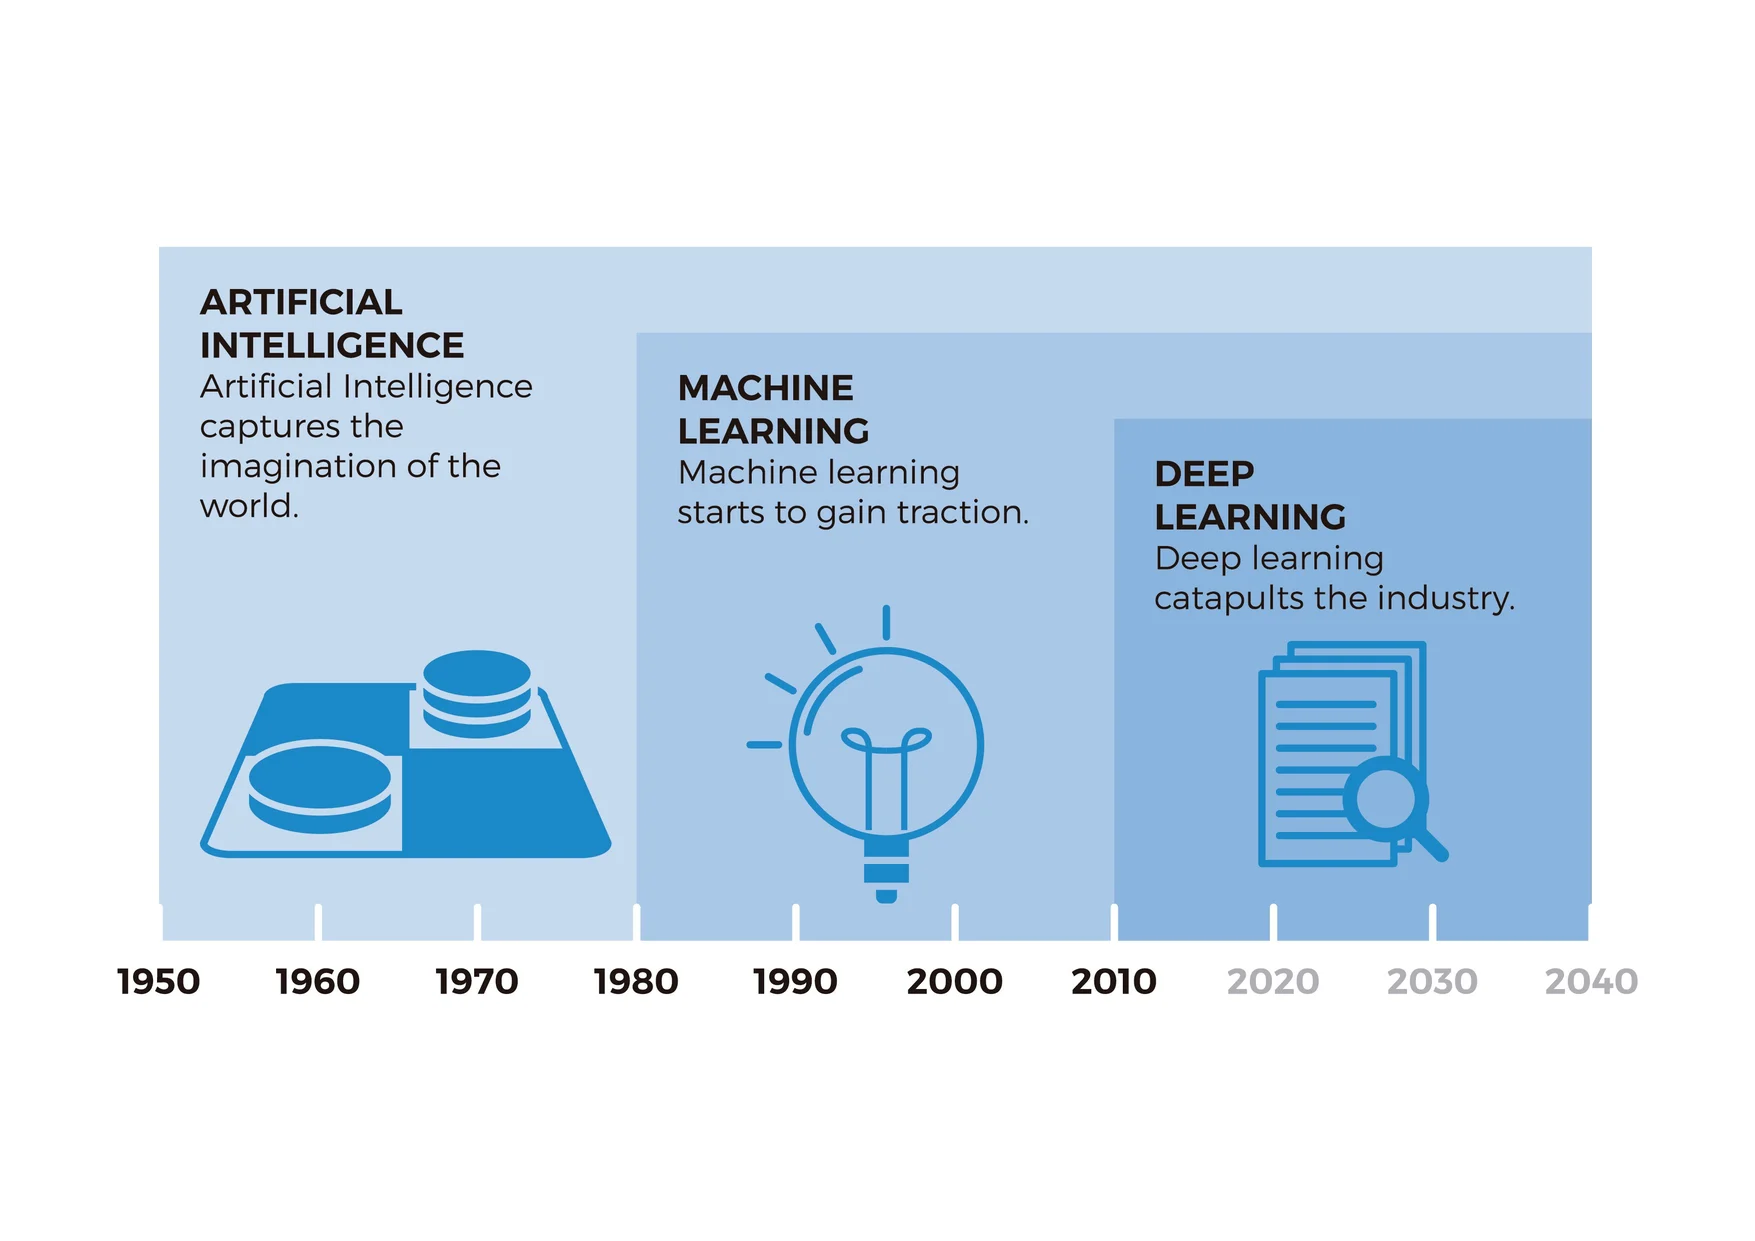
\includegraphics[width=0.8\linewidth]{MLDLevol}
        \caption{Evolution of AI, ML and DL. Source \href{https://blog.bismart.com/diferencia-machine-learning-deep-learning}{BISMART}.}
        \label{Fig:MLDLevol}
    \end{figure}
\end{frame}

\begin{frame}{Supervised ML}
    \begin{figure}
        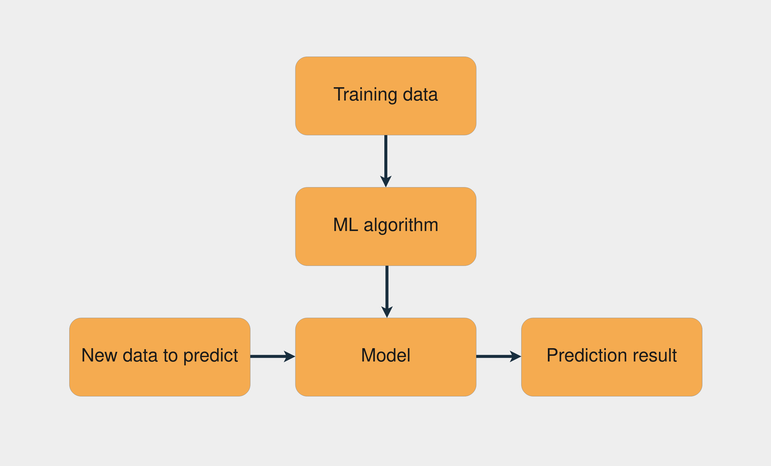
\includegraphics[width=0.9\linewidth]{ML}
        \caption{\href{https://realpython.com/python-ai-neural-network/}{Workflow} to train a model using supervised learning.}
        \label{Fig:ML}
    \end{figure}
\end{frame}

\begin{frame}{Supervised ML\cite{kroese2020}}
    \begin{itemize}
        \item Build models capable of learning from a series of data $X$.
        \item The learning process depends on the task we want to train the model:
            \begin{description}
                \item[Supervised] the input data $X$ is accompanied by the values ​$​y$ that we want the model to learn or also called targets (linear regression, decision trees, ...). The objective is that the prediction of the model given some data $x$ is equal to the target. 
                \item[Unsupervised] the task to be learned is some type of association of the input data $X$ with each other (i.e clustering).
            \end{description}
        \end{itemize}
\end{frame}


\begin{frame}{Feature engineering}
    \begin{figure}
        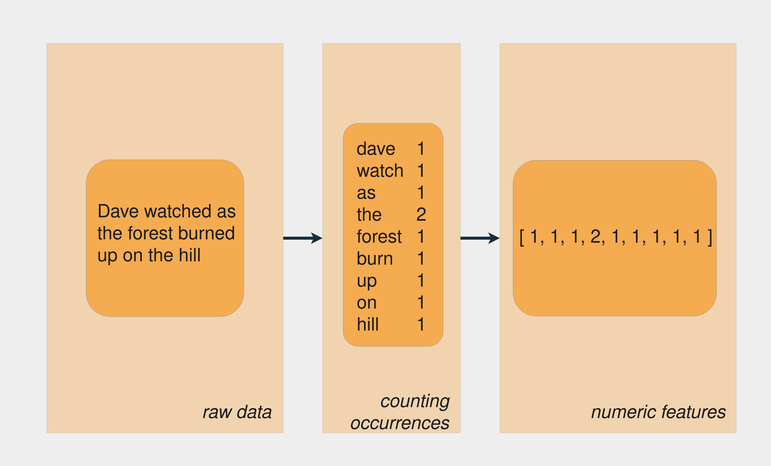
\includegraphics[width=0.9\linewidth]{FeatureEngineering}
        \caption{Feature engineering \href{https://realpython.com/python-ai-neural-network/}{example}.}
        \label{Fig:FeatureEngineering}
    \end{figure}
\end{frame}

\begin{frame}{Neural networks}
    \begin{itemize}
        \item In the ML example above, we use lemmatization to eliminate inflection from words, generating a simpler model.
        \item In neural networks, {\bf we leave the network itself} to find out the most important features in the data, without relying on feature engineering techniques. 
    \end{itemize}
    Neural Networks \href{https://towardsdatascience.com/deep-learning-with-python-neural-networks-complete-tutorial-6b53c0b06af0}{are based on} a collection of connected units (neurons), which, just like the synapses in a brain, can transmit a signal to other neurons, so that, acting like interconnected brain cells, they can learn and make decisions in a more human-like manner.
\end{frame}

\begin{frame}{ML vs DL}
    \begin{figure}
        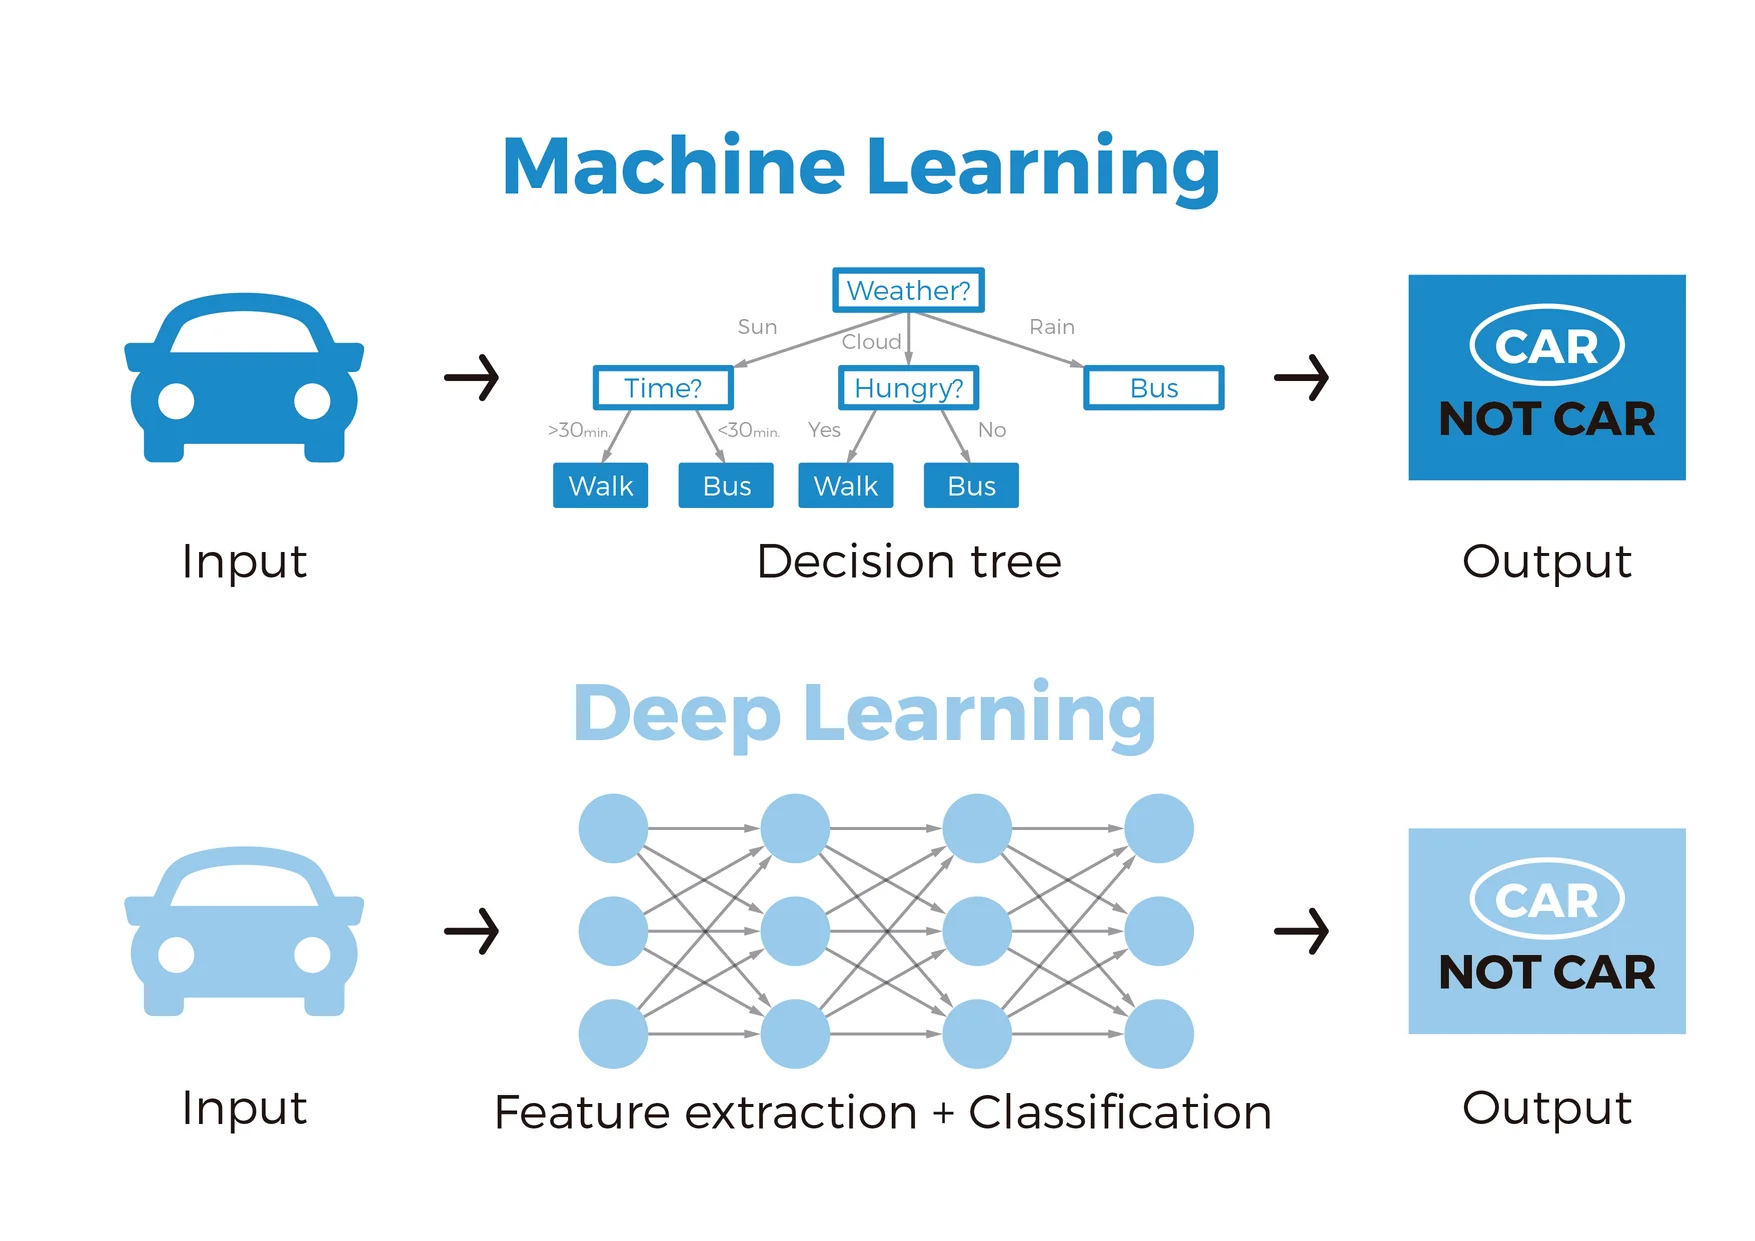
\includegraphics[width=0.8\linewidth]{MLvsDL}
        \caption{ML vs DL. Source \href{https://blog.bismart.com/diferencia-machine-learning-deep-learning}{BISMART}.}
        \label{Fig:MLvsDL}
    \end{figure}
\end{frame}

\begin{frame}{Neural networks}
    \begin{figure}
        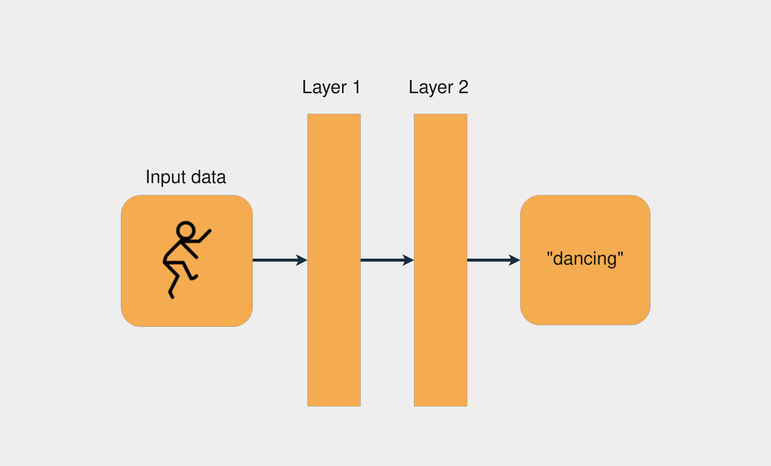
\includegraphics[width=0.9\linewidth]{2layerNN}
        \caption{ \href{https://realpython.com/python-ai-neural-network/}{Schema} of a 2 layer neural network.}
        \label{Fig:FeatureEngineering}
    \end{figure}
\end{frame}

\begin{frame}{Throwing darts and improving by learning}
    \begin{figure}
        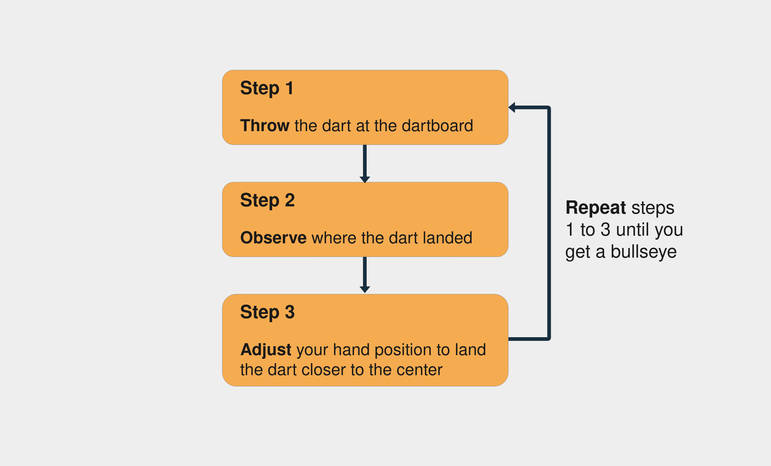
\includegraphics[width=0.9\linewidth]{TrainingDart}
        \caption{\href{https://realpython.com/python-ai-neural-network/}{Steps} for trying to hit the center of a dartboard.}
        \label{Fig:TrainingDart}
    \end{figure}
\end{frame}


\begin{frame}{Artificial Neural Networks (ANN)}
    \begin{itemize}
        \item ANN are formed by layers of neurons.
        \item Each layer has a certain number of neurons.
        \item The input data $X$ enters through the first layer and through mathematical operations the input values are transformed into output values $y'$.
        \item The goal of the network is to modify the mathematical operations through some parameters (weights and biases, $W$ and $b$) to minimize the difference bewteen $y$ and $y'$.
        \item Deep Learning refers to all those models that use ANN of any type with multiple layers.
    \end{itemize}
\end{frame}



\begin{frame}{Perceptron}
    \begin{figure}
        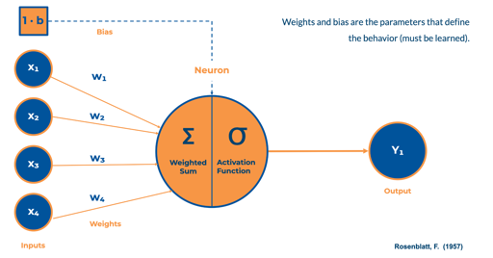
\includegraphics[width=0.9\linewidth]{perceptron}
        \caption{$w_1 x_1 + w_2 x_2 +w_3x_3+w_4x_4 \leq \mathrm{threshold} \Rightarrow Y=0$. We can introduce bias and a given function: $\sigma(\uvec{w}\cdot \uvec{x}+b)=y'$. Adpated from \cite{rosenblatt_perceptron_1958}.}
        \label{Fig:perceptron}
    \end{figure}
\end{frame}

\begin{frame}{Multilayer perceptron}
    \begin{figure}
        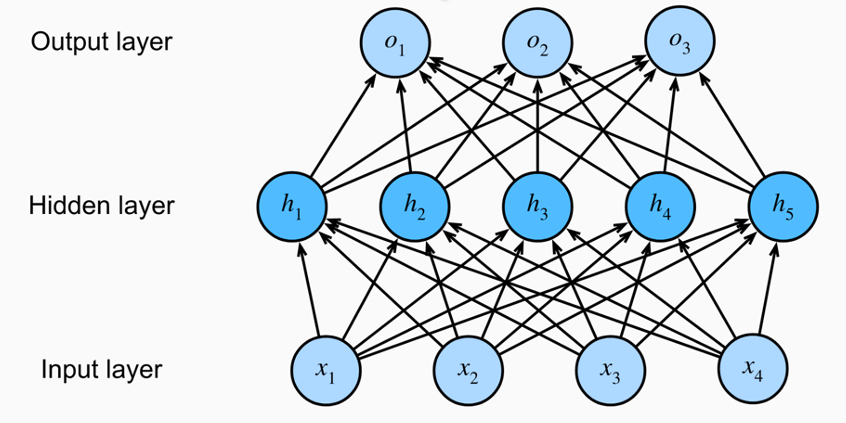
\includegraphics[width=0.9\linewidth]{MLP}
        \caption{A multilayer perceptron with 5 hidden units.}
        \label{Fig:perceptron}
    \end{figure}
\end{frame}

\begin{frame}{Multilayer perceptron: some maths}
    \small
    \[
        w^{L}_{ij}, \,
        \begin{cases}
            L = \mathrm{layer \ number} \\
            i = \mathrm{neuron \ from \ previous \ layer}\\
            j = \mathrm{neuron \ from \ following \ layer}  
        \end{cases}
    \]
    \[
        \sigma_1\left(\uvec{W}^{(1)^T} \cdot \uvec{X} + \uvec{b}^{(1)}\right) = 
        \sigma_1\left(
            \begin{bmatrix}
            w^{(1)}_{11} & w^{(1)}_{12} & w^{(1)}_{13} & w^{(1)}_{14}\\
            w^{(1)}_{21} & w^{(1)}_{22} & w^{(1)}_{23} & w^{(1)}_{24}\\
            w^{(1)}_{31} & w^{(1)}_{32} & w^{(1)}_{33} & w^{(1)}_{34}\\
            w^{(1)}_{41} & w^{(1)}_{42} & w^{(1)}_{43} & w^{(1)}_{44}\\
            w^{(1)}_{51} & w^{(1)}_{52} & w^{(1)}_{53} & w^{(1)}_{54}
            \end{bmatrix}
            \cdot
            \begin{bmatrix}
            x_{1}\\
            x_{2}\\
            x_{3}\\
            x_{4}
            \end{bmatrix}
            +
            \begin{bmatrix}
            b^{(1)}_{1}\\
            b^{(1)}_{2}\\
            b^{(1)}_{3}\\
            b^{(1)}_{4}\\
            b^{(1)}_{5}
            \end{bmatrix}
        \right) = 
        \uvec{H}^{(1)}
    \]
    \[
        \sigma_2\left(\uvec{W}^{(2)^T} \cdot  \uvec{H}^{(1)} + \uvec{b}^{(2)}\right)= 
        \sigma_2\left(\begin{bmatrix}
                w^{(2)}_{11} & w^{(2)}_{12} & w^{(2)}_{13} & w^{(2)}_{14} & w^{(2)}_{15}\\
                w^{(2)}_{21} & w^{(2)}_{22} & w^{(2)}_{23} & w^{(2)}_{24} & w^{(2)}_{25}\\
                w^{(2)}_{31} & w^{(2)}_{32} & w^{(2)}_{33} & w^{(2)}_{34} & w^{(2)}_{35}\\
                \end{bmatrix}
                \cdot
                \begin{bmatrix}
                h_{1}\\
                h_{2}\\
                h_{3}\\
                h_{4}\\
                h_{5}\\
                \end{bmatrix}
                +
                \begin{bmatrix}
                b^{(2)}_{1}\\
                b^{(2)}_{2}\\
                b^{(2)}_{3}\\
                \end{bmatrix}\right) 
                = \uvec{Y}^{\mathrm{out}}                    
    \]
    \normalsize
\end{frame}

\begin{frame}{Multilayer perceptron: some details}
    \begin{itemize}
        \item The MLP is the simplest neural network
        \item Weights connect neurons from an inner to an outer layer
        \item Operations in each layer are implemented using matrices and vectors
        \item The {\bf forward pass} of the last layer produces the ouput.
        \item The MLP can be interpreted as a multivariant function with $W$ and $b$ as the parameters, $X$ as input and $Y^{\mathrm{out}}$ as output.
        \item {\bf Hiperparameters} are additional parameters that control other aspects: number of layers, number of neurons per layer, acivation functions, ...
    \end{itemize}
\end{frame}

\begin{frame}{The logistic function}
    \begin{figure}
        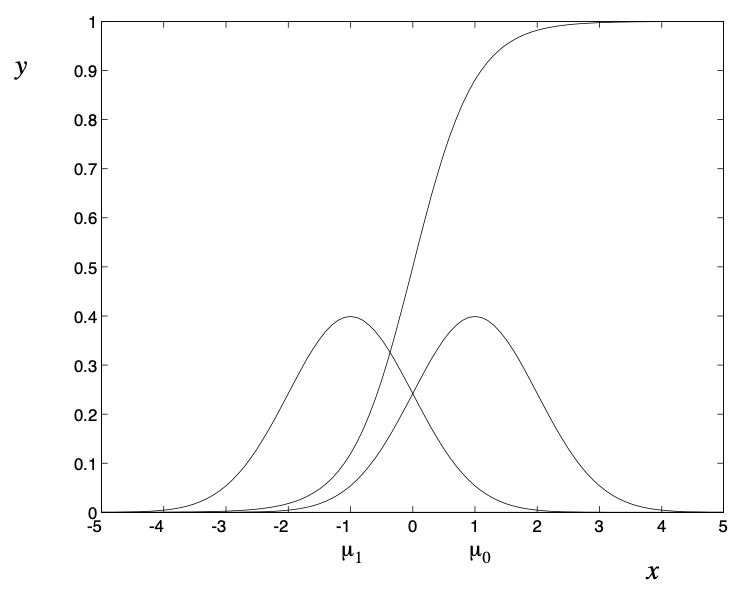
\includegraphics[width=0.6\linewidth]{logistic}
        \caption{A binary classification problem. The class-conditional densities are Gaussians with unit $\sigma^2$. The posterior probability is the logistic function $y=1/(1+\exp{(-2x)})$\cite{jordan_why_1995}.}
        \label{Fig:logistic}
    \end{figure}
\end{frame}

\begin{frame}{Activation functions}
    \begin{columns}
        \begin{column}{0.4\linewidth}     
            \href{https://machinelearninggeek.com/activation-functions/}{Activation functions}:
            \begin{itemize}
                \item The {\bf sigmoid} function is used in the final layer in classification models.
                \item {\bf ReLU} is used in inner layers, as they produce non-linerity.
                \item All are differentiable. 
            \end{itemize}
        \end{column}
        \begin{column}{0.6\linewidth}
            \begin{figure}
                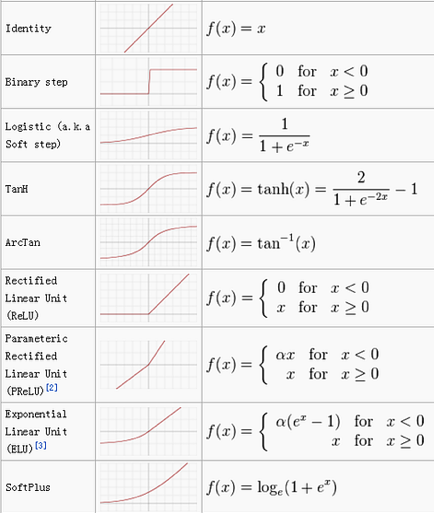
\includegraphics[width=0.8\linewidth]{activationfunctions}
            \end{figure}
        \end{column}
     \end{columns}
\end{frame}



\begin{frame}{An example of a 2 layer Neural Network}
    \begin{columns}
        \begin{column}{0.6\linewidth}     
            Example of classification (for categories "1" and "0") with a 2 layers NN. 
            \begin{itemize}
                \item In the first layer we use a linear regression approach.
                \item The second layer includes the non-linearity through the use of a \href{https://en.wikipedia.org/wiki/Sigmoid_function}{sigmoid function} that decides whether the prediction is 1 or 0, following the \href{https://en.wikipedia.org/wiki/Bernoulli_distribution}{Bernouilli distribution}.
            \end{itemize}
        \end{column}
        \begin{column}{0.4\linewidth}
            \begin{figure}
                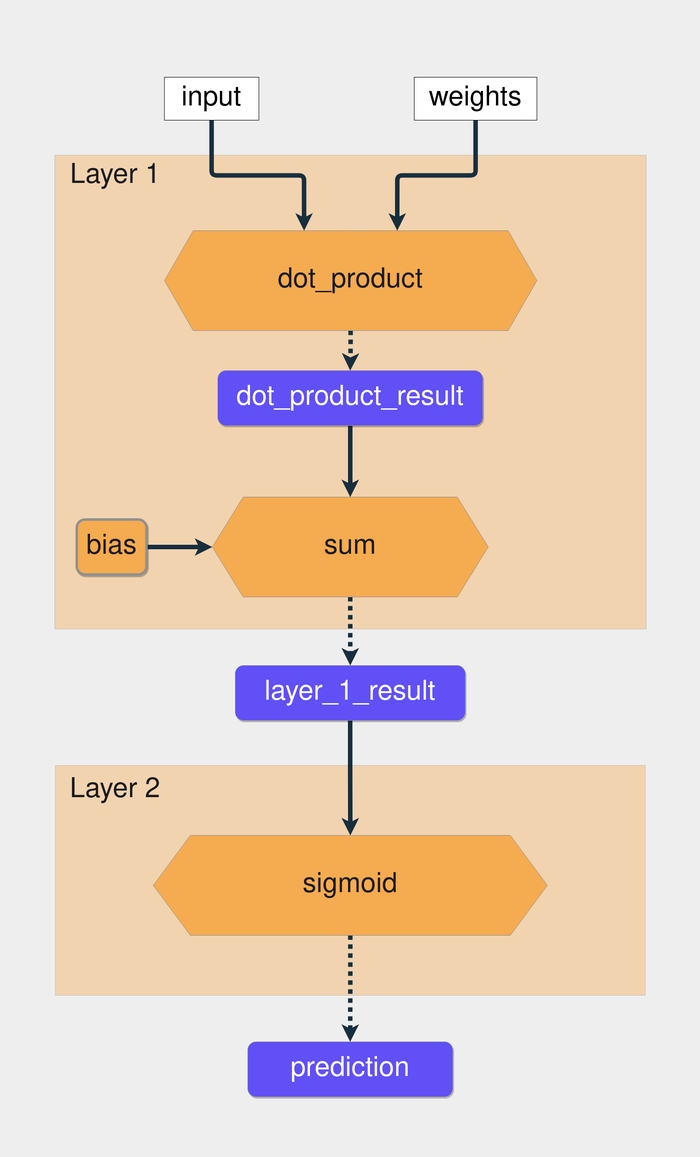
\includegraphics[width=0.7\linewidth]{Training2Layer}
                \caption{\href{https://realpython.com/python-ai-neural-network/}{Training} a two layer neural network.}
                \label{Fig:Training2Layer}
            \end{figure}
        \end{column}
     \end{columns}
\end{frame}




\begin{frame}
    \begin{Exercise}{Loss/Cost function in a simple 2 layer NN}
        \label{Ex:2layer}
        Check the \href{https://github.com/Biocomputing-Teaching/Data-Science-with-Python/blob/main/code/UNIT9-Neural-Networks.ipynb}{provided code} for this session and expand it to:
        \begin{enumerate}
            \item Generate a collection of 100 synthetic data points from a two Gaussian distribution.
            \item Assign the data points a category "0" or "1" depending on the Gaussian function they are obtained from.
            \item Use the provided 2 layers NN to evaluate the expected value of the loss function with the provided weights.
            \item Can you guess the weights that would improve the prediction (reducing the value of the error)?
        \end{enumerate}
    \end{Exercise}
\end{frame}

\begin{frame}[fragile]{Backpropagation: weights}
    \begin{columns}
        \begin{column}{0.6\linewidth}     
            {\bf Chain Rule in Backpropagation}In each {\bf backward pass}, you compute the partial derivatives of each function, substitute the variables by their values, and finally multiply everything.
            \\[10pt]
            Notice that, for the sigmoid function $f(x)=\frac{1}{1+e^{-x}}$, $f'(x)=1-f(x)$.
            \\[10pt]
            \begin{lstlisting}[language=Python]
derror_dweights = 
derror_dprediction 
* dprediction_dlayer1 
* dlayer1_dweights
            \end{lstlisting}
        \end{column}
        \begin{column}{0.4\linewidth}
            \begin{figure}
                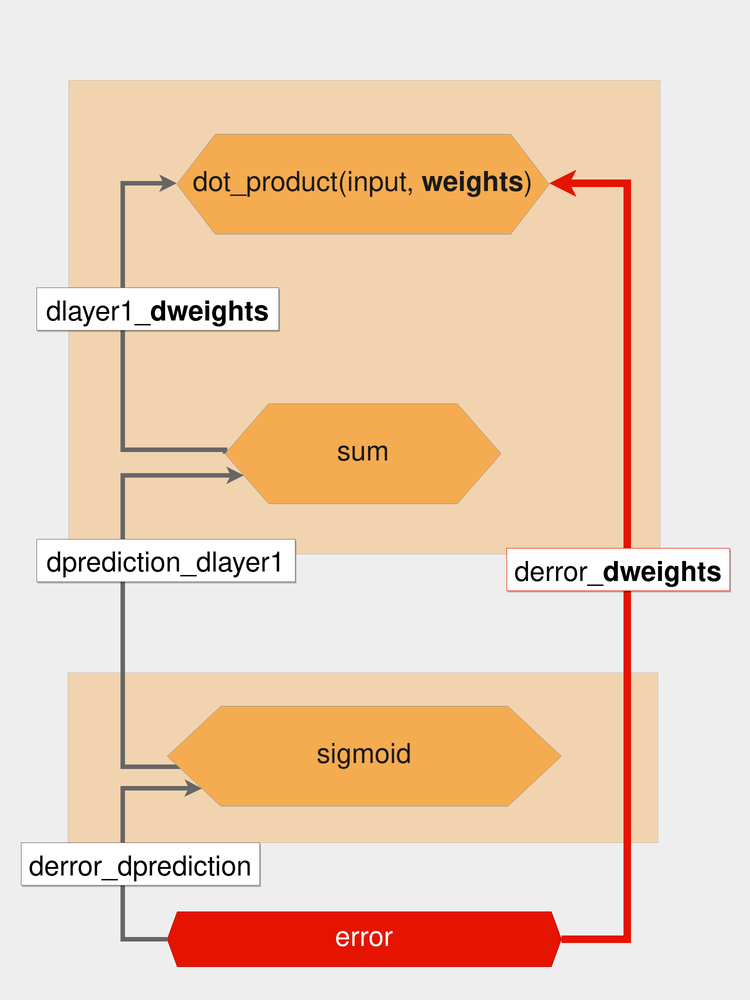
\includegraphics[width=0.9\linewidth]{WeightGradient.png}
                \caption{\href{https://realpython.com/python-ai-neural-network/}{Chain rule:}  derivative of the  error with respect to {\bf weights}.}
                \label{Fig:Training2Layer}
            \end{figure}
        \end{column}
     \end{columns}
\end{frame}

\begin{frame}[fragile]{Backpropagation: bias}
    \begin{columns}
        \begin{column}{0.6\linewidth}  
            Chain rule applied to the derivative of the bias error in the 2 layer example.   
            \begin{lstlisting}[language=Python]
derror_dbias =  derror_dprediction 
* dprediction_dlayer1 
* dlayer1_dbias
            \end{lstlisting}
        \end{column}
        \begin{column}{0.4\linewidth}
            \begin{figure}
                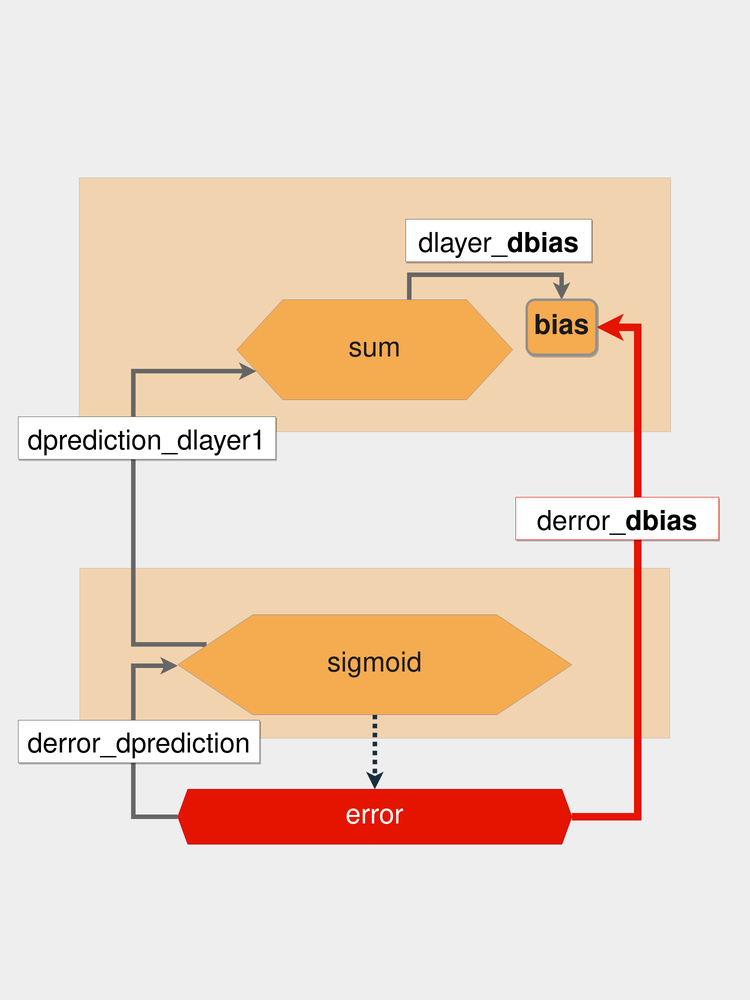
\includegraphics[width=0.9\linewidth]{BiasGradient}
                \caption{\href{https://realpython.com/python-ai-neural-network/}{Chain rule:}  derivative of the error with respect to {\bf bias}.}
                \label{Fig:Training2Layer}
            \end{figure}
        \end{column}
     \end{columns}
\end{frame}


% nous temes:
% -encoding/decoding
% -RFECV
% -computer vision
% -training NN (iceland 8)
% -CNN (iceland 9)
% -GAN
% -tensorflow vs pytorch vs keras
% -recommender

\section{Bibliography}
\bibliographystyle{unsrt}
\bibliography{DataSciencewithPython}
\end{document}
